\graphicspath{ {6-Experimento/} }

\chapter{O Experimento}

Como mencionado no Capítulo \ref{sgbd}, muitas empresas ainda utilizam 
bancos relacionais como forma de gerenciar seus dados. Existem vários SGBDR 
atuantes no mercado, como MySQL, PostgreSQL e algumas variantes da Oracle. 
Por se tratar de um SGBD \textit{open source} e ser amplamente 
conhecido, foi escolhido para o estudo o PostgreSQL. Ele possui vasta 
documentação, tutoriais e suporte em fóruns sobre bancos de dados e 
programação de forma geral, além de receber recorrentes atualizações. 

A categoria de NoSQL escolhida foi a colunar, por ser a mais 
recomendada para gerenciamento do grande volume de dados de um DW. 
O fato do PostgreSQL utilizar a Linguagem SQL como forma de 
manipulação de dados faz com que seja necessário também escolher 
o banco colunar para comparação utilizando esse filtro. A escolha também 
se deu com base na simplicidade do uso do SGBD, e na praticidade de 
migração dos dados armazenados entre um banco e outro. Para tanto, 
o MonetDB foi definido para o estudo.

O gerenciamento dos SGBD foi realizado através do \textit{driver} JDBC 
disponibilizados nas páginas oficiais do PostgreSQL e do MonetDB. Seu uso se deu 
devido à simplificação no desenvolvimento de aplicações, por dar suporte a 
diferentes SGBD e possuir boa documentação e tutoriais. Na análise de tempo 
foi considerada a latência da Máquina Virtual Java (JVM), assim incluindo essa 
latência no tempo total. As versões dos SGBD utilizadas 
foram o PostgreSQL 9.6 e o MonetDB XXX e foram instalados no servidor do laboratório GIA, operando o 
sistema operacional Ubuntu Linux 16.04 LTS, com 16Gb de RAM e dois 
processadores Intel Xeon CPU E5620 2.40GHz.

Os cenários de teste consistiram de três bases de dados de tamanhos 
diferentes, de 1Gb, 10Gb e 30Gb para simular desde uma base pequena 
até bases maiores. Cada cenário foi executado nos ambientes \textit{snowflake} e 
\textit{star}.

Alguns fatores devem ser considerados ao executar testes de \textit{benchmark} 
no escopo de banco de dados \cite{raasveldt2018fair}:

\begin{enumerate}
    \item{O ambiente de execução 
    deve ser o mesmo para todos os SGBD, bem como a lógica e sequência de 
    execução.}
    \item{A modelagem do banco deve ser idêntica para todos os modelos, e isso 
    inclui os tipos de dados e restrições de integridade. Ao analisar os resultados do \textit{benchmark}, a menos 
    que seja especificado no estudo, não há como saber qual é o tipo de dado de um atributo 
    quando existem diferentes tipos que podem ser usados para a mesma função, 
    e essa diferença acarreta em resultados diferentes de desempenho. Por exemplo, 
    em Raasveldt et al. \cite{raasveldt2018fair} o SGBD MariaDB apresentou diferenças quando implementado 
    utilizando DECIMAL e DOUBLE.}
    \item{\textit{Cold run} vs. \textit{Hot run}: em alguns sistemas a primeira execução de 
    testes (\textit{cold}) costuma levar mais tempo para executar que as execuções subsequentes (\textit{hot}). 
    Isso se dá pelo buffer do banco de dados ou o próprio sistema operacional ter armazenado em 
    cache os dados requeridos.}
\end{enumerate}

Os itens 1 e 2 foram tratados antes da execução do TPC-H. Nos Apêndices \ref{ddl_snow} e \ref{ddl_star} se encontram as SQL 
utilizadas para criar os esquemas \textit{snowflake} e \textit{star} nos SGBD. O fluxograma da Figura \ref{fig:flux} 
ilustra ainda a sequência de passos desde a criação dos bancos até a execução do \textit{benchmark}. 

O item 3 foi tratado durante a execução das consultas do teste de força: para cada cenário é realizada três 
análises diferentes, a primeira considerando a primeira execução de consultas; a segunda considerando o melhor 
resultado entre três execuções; e a terceira limpando parte da cache do sistema operacional antes de 
rodar a terceira execução. Essa análise é feita somente sob as consultas do teste de força por ser o primeiro 
teste a ser feito, como pode ser observado na Figura \ref{fig:power_flux}, que ilustra o fluxograma do teste de força. No teste de vazão todas as consultas já foram executadas 
uma vez e as funções de atualização trabalham sobre dados diferentes a cada vez que são executadas, impossibilitando 
o armazenamento em cache.

\begin{figure*}[htpb]
	\centering
        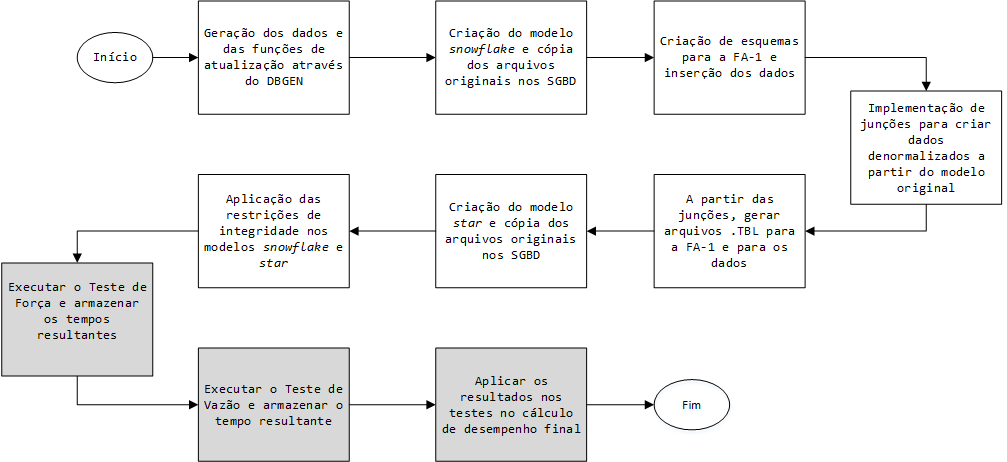
\includegraphics[width=\textwidth]{flux}
	\caption{Fluxograma do desenvolvimento até o cálculo final de desempenho do TPC-H}
	\label{fig:flux}
\end{figure*}

\begin{figure*}[htpb]
	\centering
        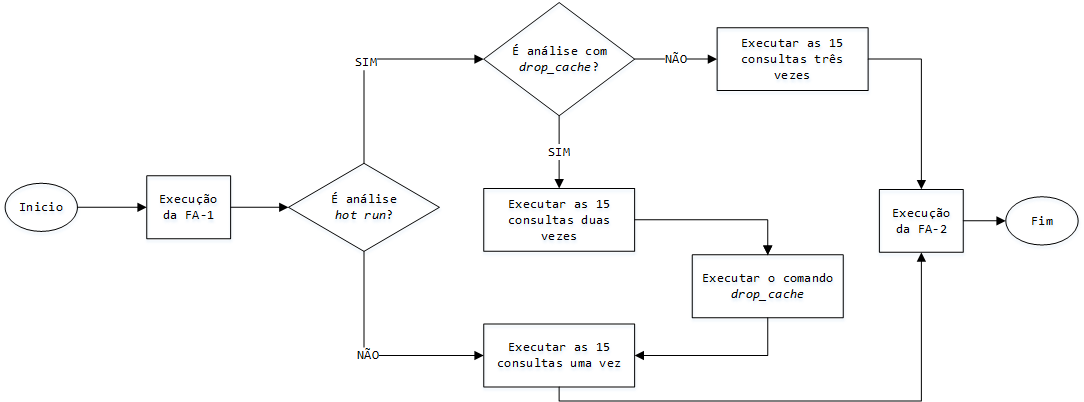
\includegraphics[width=\textwidth]{power_flux}
	\caption{Fluxograma do desenvolvimento do teste de força considerando todas as variações de cenário}
	\label{fig:power_flux}
\end{figure*}

Para averiguar se todas as 22 consultas do TPC-H executam de forma correta e em tempo hábil, principalmente 
atentando-se ao fato de que no ambiente denormalizado elas foram modificadas, foi realizada uma execução 
prévia de cada uma, sob a menor base de dados, utilizando o JDBC. Dessa execução, foram eliminadas as consultas 
Q1, Q2, Q4, Q15, Q17, Q20 e Q21 por terem demorado horas no ambiente denormalizado -- e algumas tendo a execução 
cancelada antes -- enquanto que as demais levaram apenas alguns segundos para executar. Essa mudança no número 
de consultas fez com que as equações originais fossem adaptadas para a nova quantidade, 15.

\begin{myequation}%
\label{eq:1-2}
{\scriptstyle Power@Size} = \frac{3600 * SF}{\sqrt[17]{\prod_{i = 1}^{i = 15}Q(i, 0) * \prod_{j = 1}^{j = 2}RF(j, 0)}} %
\end{myequation}
%

\begin{myequation}%
\label{eq:2-2}
{\scriptstyle Throughput@Size} = \frac{S * 15 * 3600}{T_s * SF} %
\end{myequation}
%

\section{Carregamento de Dados}



\section{Base de 1GB}

\section{Base de 10GB}

\section{Base de 30GB}

